\documentclass[11pt]{article}
\usepackage[margin=.85in]{geometry}
\usepackage[T1]{fontenc}
\usepackage{amsmath,graphicx,booktabs,longtable,array,hyperref}
\hypersetup{colorlinks=true,urlcolor=blue,linkcolor=blue}
\setlength{\emergencystretch}{3em}
\title{Independent observations, provisional association, and limits to reproducing the Campi Flegrei catalog}
\author{Reproduction assessment of Tan et al. (2025)}
\date{9 October 2026}
\begin{document}\maketitle
% All numerical results are read from executed output files.

\begin{abstract}
Tan et al. describe an observational earthquake-catalog workflow, not a coupled physical forward model. This resumed investigation processes original waveforms, applies the released retrained PhaseNet model, runs provisional GaMMA association with an explicitly different external starting profile, and attempts response-corrected relative-magnitude measurements. It also recovers original leveling and GNSS observations. No publication panel is fully independently reproduced. Figure 1B and supplementary S1, S2 and S15C are partial; external routine-catalog context is shown separately. The complete multiyear acquisition, calibrated locations, double-difference relocation, magnitude distribution and focal mechanisms remain incomplete. A successful rebuild establishes execution of the reported limited calculations, not reproduction of unexecuted stages.
\end{abstract}

\section{Scientific specification and input verification}
The local \path{tanmodel.pdf} and \path{tanmodelsupp.pdf} were extracted before changing outputs. Main captions 1--4, supplementary captions S1--S15 and methods S2--S11 are readable. Two font-weight warnings do not prevent main-text extraction. Both supplied ZIPs were listed and CRC-tested; no file from them was executed. Their inventory and hashes are in \path{docs/resumed_source_check.json} and \path{docs/file_inventory.json}.
\begingroup\small\begin{longtable}{p{.52\linewidth}r p{.25\linewidth}}
\toprule
File & Bytes & Inspection\\\midrule
\endhead
\path{tanmodel.pdf} & 2140554 & Text and captions readable\\[3pt]
\path{tanmodelsupp.pdf} & 62164947 & Text and captions readable\\[3pt]
\path{science.adw9038_data_s1_to_s3.zip} & 12960255 & Directory readable; CRC passed; not executed\\[3pt]
\path{science.adw9038_interactive_plot_s1.zip} & 8852485 & Directory readable; CRC passed; not executed\\[3pt]
\bottomrule
\end{longtable}
\endgroup
The data archive contains Data S1 (final event catalog), S2 (associated phases) and S3 (focal mechanisms), plus binary macOS packaging metadata. The other archive contains an HTML seismicity visualization. These are derived products, not original waveform inputs. Data S1 was read only after independent outputs existed, for a separate final comparison of temporal coincidences and horizontal differences. Data S3 was read only for a final row-count audit: the CSV has 74 rows and 58 nonempty gCAP solutions, consistent with the methods. Its caption's 55-event description is inconsistent with the actual file. No supplied solution entered inference, initialization, filtering or magnitude estimation.

The latest instruction permits an external input genuinely required by the published method. Accordingly, routine INGV duration magnitudes are permitted only after independent detection and association, as supplementary S6's explicit magnitude regularization reference. Their use no longer presents the blanket policy conflict stated in the previous report. The picking/association program never opens that catalog. Historical catalog plots are explicitly external context, not independently detected earthquakes.

The authors' fitted 1D velocity model, station corrections, picks, associated catalog, focal solutions and study scripts remain excluded. Generic PhaseNet/SeisBench, GaMMA and VELEST are attributed method software. The trained PhaseNet artifact is used for new inference; retraining is not claimed. All numerical figures read saved CSV or NPZ outputs. No figure was digitized, and no published image substitutes for an output.

\section{Data access and actual coverage}
The frozen rebuild snapshot contains 230 external files (435,600,234 bytes). Original and extended processing read 171 waveform files from 26 stations, representing 428.983 channel-hours after unioning overlapping intervals. This is a lower bound on retrieved coverage, not a full-network availability estimate.

The study interval is 21 January 2022 through 20 March 2025. All 26 full-period IV/2I station requests returned HTTP 413, explicitly citing a one-billion-sample limit. This is a request-size constraint, not evidence that the archive is unavailable. Half-hour requests were then executed for calendar-selected windows on 21 January 2022, 1 January 2023, 1 January 2024 and 20 March 2025. These windows were chosen independently of every earthquake catalog. Daily requests were also attempted; most timed out after 180 seconds, while two returned complete files. Failed transfers are not counted as full-day coverage. A resumable retrieval tool and exact input manifest accompany the project. Full-period download and processing remain unfinished.

Complete response metadata was obtained for 26 station names in networks IV and 2I. This extends the previous four-station response inventory and includes four temporary-network stations. Metadata epochs do not prove continuous recording. The coverage figure uses returned miniSEED segments and preserves gaps. Coverage totals count each channel separately; they do not imply three-component coverage throughout every station interval. Some single-channel records do not support the three-component picker. Actual input files, channel segments, sampling rates, and unioned intervals are saved in the manifests and coverage tables.

The INGV landing page fails local TLS issuer verification, whereas the official FDSN service works with normal verification. RAN's public pages are readable but waveform downloads require registration/login; credentials were unavailable. No account was created. Individual HTTP 204, HTTP 502 and timeout results remain explicit in the receipt files.

The temporary/local ZIP's directory was read using HTTP byte ranges. It lists 319,890 members and approximately 3.845 GB of uncompressed content. Its actual filename station inventory includes CFB1, CFB3, CROS, V0102, V0105, CRUS and CMDP; it does not establish every station advertised on the landing page. One miniSEED member was read successfully, with 6001 samples over 60 seconds. These observations are cut around author-detected events and therefore cannot supply unbiased continuous event discovery. They were not used to seed analysis. The four 2I stations were instead accessed through continuous FDSN requests.

\section{Independent processing and explicit departures}
\subsection{Picking and provisional association}
The picker uses released tensors with a strict tensor-only load, 100 Hz sampling, nominal 30-second windows, ENZ components, standard-deviation normalization, 1500-sample overlap, 250-sample edge blinding and a 0.3 P/S threshold. The release README specifies a 1 Hz highpass; four poles and a causal implementation are explicit choices. Extended processing uses 30-minute cores with 15-second context where recorded. Missing intervals are not interpolated. Repeated picks within 0.25 seconds at the same station and phase are merged by retaining the larger score. This merging tolerance is an assumption. S picks at CASE, CFB1 and CFB3 are excluded.

The numerical starting profile cited by the paper is Cal\`o and Tramelli (2018). Its retrieved supplement presents that profile graphically; no numerical table was found, and its data statement offers data on request. No plot was digitized. The released fixed 3D file is identified in the model repository as the TomoDD input; the paper attributes its fixed background to Battaglia et al. (2008). Its original-release byte identity remains unverified. The file contains a $23\times14\times27$ grid of $V_P$ and $V_P/V_S$; $V_S$ is calculated by division before averaging.

Two independent horizontal averages were computed: 14.02--14.20 degrees E, 40.77--40.86 degrees N, and a central box at 14.11--14.16 degrees E, 40.81--40.84 degrees N. These polygons are explicit assumptions, not inferred figure borders. Bounding nodes and the deep 200 km padding level are omitted from the association profile. Above sea level, the surface velocity is extended to station elevations rather than averaging air nodes. This profile is a sensitivity alternative; the associated events cannot be called an exact reproduction of the paper's first locations.

GaMMA uses its 1D eikonal travel-time option with 0.1 km grid spacing. The association requires at least six picks, without separate P/S minima. Additional declared settings are a 10-second DBSCAN neighborhood, three minimum DBSCAN samples, fivefold mixture oversampling, a time-only likelihood, 1 second-squared covariance prior, horizontal bounds of $\pm12$ km and depth bounds of 0--8 km. Amplitude is omitted from association because the paper does not specify its association-amplitude configuration; the GaMMA placeholder magnitude is removed from saved events. These choices are in \path{config/association.json} and were not tuned against a supplied catalog.

\subsection{Location quality and magnitude attempt}
Travel-time residuals are recomputed from each provisional origin and the same eikonal model. I calculate
\[
R=\sqrt{\frac{1}{N}\sum_{k=1}^{N}(t_k-t_0-T_k)^2},
\]
and the largest unoccupied azimuth between distinct stations. The generic VELEST guidance requires more than six observations and a gap below 180 degrees for calibration candidates. This is a geometry screen, not acceptance of their waveform interpretations. The paper's 0.25-second rejection is a post-location criterion and is not imposed prematurely as a calibration prerequisite.

The generic VELEST source builds after three platform-only repairs: a FORMAT trailing comma, the CPU clock, and the date/time routine. Its scientific inversion was not run. The small provisional candidate set does not constrain the chosen 21-level P/S model, hypocenters and station corrections. The paper used 373 calibration events. No author-fitted model fills this gap. Consequently, the prescribed VELEST residual-rejection sequence, two TomoDD rounds and regional HypoDD SVD uncertainty tests remain unexecuted.

The magnitude attempt nevertheless measures available waveforms independently for all provisional events, without restricting it to the VELEST calibration subset. A recorded P pick defines the arrival, with the calculated P arrival used where only S is assigned. Full response removal produces velocity with a 0.1, 0.2, 35, 45 Hz prefilter and 60 dB water level; these are stated measurement assumptions, not fully specified publication settings. Signal and noise powers use five seconds after and two seconds before the arrival:
\[
\mathrm{SNR}=10\log_{10}(P_{\rm signal}/P_{\rm noise}).
\]
Observations below 5 dB are rejected. Candidate event pairs require at least two common stations and separation below one-fifth of both source--station distances. The measured equation is
\[
M_i-M_j=\log_{10}(A_{is}/A_{js}).
\]
The implemented least-squares objective weights channel equations by squared waveform correlation and uses routine $M_d$ priors with declared unit regularization weight. A connected component must contain measured amplitude-difference equations and a matched external anchor. It cannot acquire a magnitude merely because an external $M_d$ exists. This run produced no qualifying edge and therefore no calibrated magnitude. Completeness and b-value cannot be estimated from an empty independently calibrated sample.

\subsection{Hybrid waveforms and search}
The three templates use the times written in supplementary S9. Matching uses eight-second CAAM/COLB vertical windows, a causal four-pole 0.2--6 Hz filter, mean two-station normalized correlation above 0.25, eight-second peak separation and exclusion of ten-second segment edges. Every supported downloaded common interval is scanned, with duplicate exposure removed. This is not a three-year search.

Candidate frequency indices use separate response-corrected, eight-second CAAM windows:
\[
\mathrm{FI}=\log_{10}(P_{8\text{--}15\,\mathrm{Hz}}/P_{2\text{--}5\,\mathrm{Hz}}).
\]
The matching bandpass is not reused for FI. Candidate waveform panels contain largely persistent broadband fluctuations and do not establish an isolated hybrid onset with a decaying low-frequency coda. All remain unconfirmed. No relative magnitude is assigned to a supposed hybrid cluster before common-source membership is established. The original three template displays remain useful observations; only the E3 example corresponds to S15C. E1/E2 displays are not S15A/B reproductions.

\section{Results, validation and comparison}
Extended inference produced 3,637 merged picks (560 P and 3,077 S). GaMMA provisionally associated 63 picks into 9 events. Only 3 events pass the stated geometry screen; none has completed independent VELEST/TomoDD processing. The magnitude attempt measured 140 channel amplitudes, 23 above 5 dB, and produced 0 qualifying equations and 0 calibrated magnitudes. Post-association external matching found 3 unique temporal matches within two seconds; these did not affect event detection or acceptance. The template search scanned 26 intervals (24.298 hours of valid start times), generating 4 unconfirmed candidates. Analytic association location error was 5.96e-07 km and origin-time error 0 s.

A strictly downstream comparison against supplied Data S1 (54,319 events) finds 5 unique temporal matches within two seconds among 9 provisional events. For these matches, the median absolute origin-time difference is 0.350 s and median horizontal difference is 1.042 km (maximum 1.730 km). These differences describe an initial, uncalibrated sample. Temporal proximity alone does not prove event identity, and unmatched events are not declared false detections. The comparison changes no independent data or setting.

The association consistency test recovers one analytically constructed homogeneous-medium event with 16 P/S arrivals. It tests association and coordinates, not earthquake-detection accuracy or the adequacy of the alternative background profile. Probability bounds, S-pick exclusions, six-pick minima and assignment uniqueness are checked. The original 27 C++ equation checks and observational waveform/FI checks are retained and rerun. All 27 checks passed. The maximum absolute FI error across the analytic mixtures was 4e-15; the maximum exact-recovery magnitude error was 1.94e-16. These errors compare against analytic fixtures, not observed earthquakes.


An additional inference comparison uses the generic original PhaseNet weights converted by SeisBench and the released retrained weights. It processes calendar-selected CSOB and CMIS observations with the same stated preprocessing. In the 1600-second CMIS window, the original model returns 17 P and 4 S picks, versus 11 P and 55 S picks from the retrained model. The waveform is dominated by persistent fluctuations. Without independently reviewed annotations, these counts establish neither greater sensitivity nor better accuracy. The 120-second CSOB window yields no original-model pick and one retrained S pick. Neither window is claimed to match S4's illustrated example. No retraining or labeled benchmark was executed. Saved probability arrays and both plots accompany the report.

The location-consistency diagnostic compares observed and calculated S--P intervals at stations with both independently assigned phases. It does not validate location accuracy independently of the fitted model. No associated CPOZ P arrival exists in this sample, so the paper's arrival-aligned CPOZ sector gathers cannot yet be formed. Counts and residuals are saved in \path{data/extended/location_consistency.json}; no author pick fills this gap.

The historical leveling calculation independently extracts 128 tabulated entries from the original Del Gaudio et al. supplement, March 1905--July 2009. It subtracts the March 1905 benchmark elevation. The resulting displacement ranges from $-1.266$ to $2.541$ m. Some source entries are estimates from photographs or earlier graphical reconstructions; their descriptions are retained. This investigation digitizes no graph. The original De Martino et al. (2021) supplement was subsequently retrieved from the publisher's static content host despite HTTP 403 on its main supplement page. Its RITE daily file supplies North, East and Up positions and uncertainties in meters, with Modified Julian Dates, through December 2019. I estimate a constant datum offset as the median difference between each overlapping leveling observation and the median GNSS Up value within 15 days. Both original series are retained; this assumes a common local displacement history and does not remove spatial differences between benchmarks. The offset and its median absolute deviation are recorded. Original daily observations for 2020--2023 remain missing. The December 2023 official monitoring bulletin gives a written approximate uplift of 1.19 m since November 2005. A separate endpoint is referenced to the median of the original November 2005 GNSS observations; no curve fills the intervening gap and no plot pixels supply values. A later interpolated compilation is excluded as a replacement.

Routine catalog pages for 2005--2025 were retrieved for explicit external context and the permitted calibration role. The current study-period download has 19,274 records, of which 12,503 have location and depth, versus 12,083 events in the publication's S5. This 420-event difference must not be removed by matching an author event list. Possible causes include archive revisions or selection differences; they are not resolved here. Context counts include unlocated events where appropriate, whereas maps require coordinates. The three-year independent detection rate, relocation precision, ring-fault geometry and magnitude-frequency distribution cannot be validated from the limited provisional sample.

After generating the displacement plot, I inspected the published Figure 1B visually. The sequence of early subsidence, uplift episodes and subsequent relaxation agrees qualitatively. The displayed vertical datum differs: the present plot subtracts the original table's March 1905 benchmark height of 3.464 m, whereas the source elevations are retained in the saved table. Absolute plot ordinates should therefore not be compared without accounting for the datum. No value was digitized or used to adjust the analysis from this comparison. The incomplete recent daily series precludes a full temporal reconstruction.

\begin{figure}[p]\centering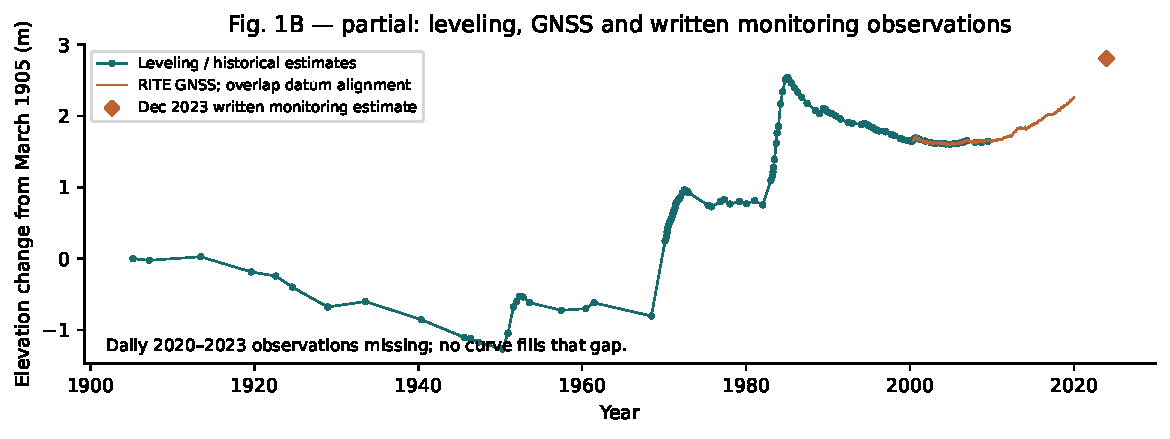
\includegraphics[width=\linewidth]{figures/historical_leveling_partial.pdf}\caption{Figure 1B, partial. Independently extracted original leveling and GNSS observations, referenced to March 1905 using the stated overlap datum alignment. Dates denote the middle of the tabulated month; uncertain months remain flagged in CSV. Leveling ends in 2009 and daily GNSS in 2019. A separate December 2023 endpoint comes from the written monitoring summary; no curve fills the daily-observation gap.}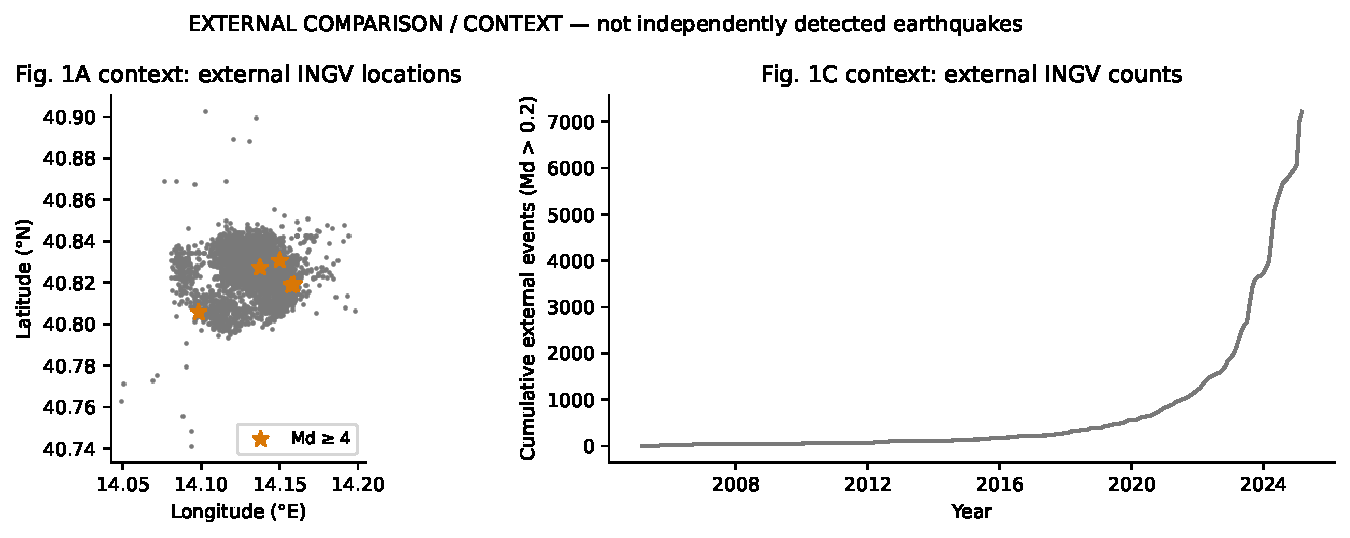
\includegraphics[width=\linewidth]{figures/historical_catalog_context.pdf}\caption{Clearly labeled external context related to Figure 1A/C. These are routine INGV events, not independently detected events. No external event is inserted into the independent association output.}\end{figure}
\begin{figure}[p]\centering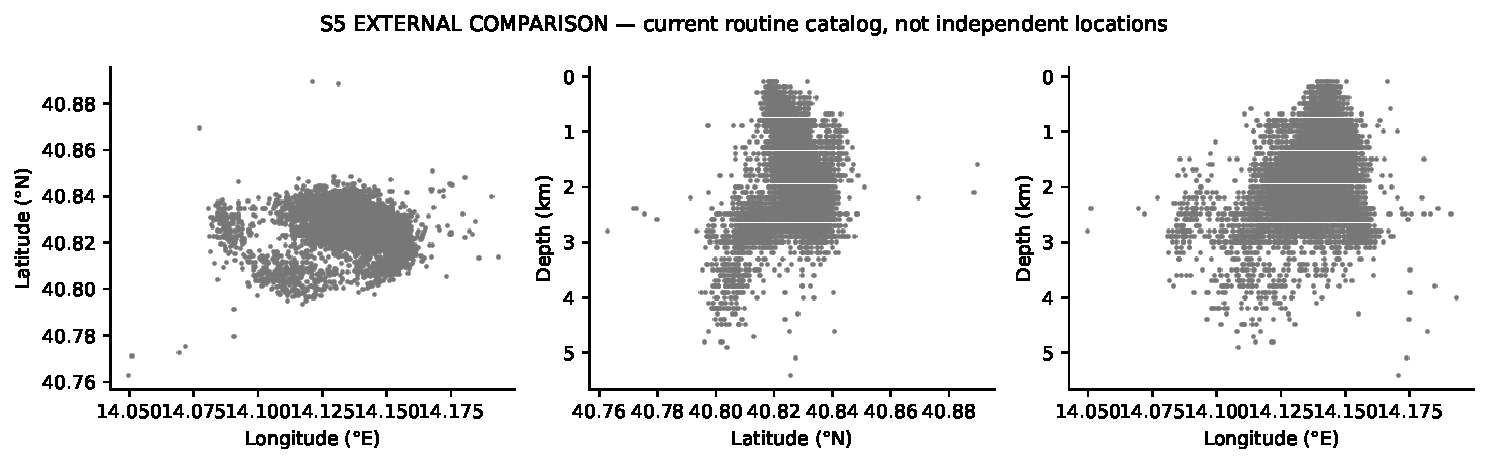
\includegraphics[width=\linewidth]{figures/routine_catalog_context.pdf}\caption{External comparison related to S5. Current routine-catalog locations during the study period; this is not an independent location result. The current located count differs from the paper.}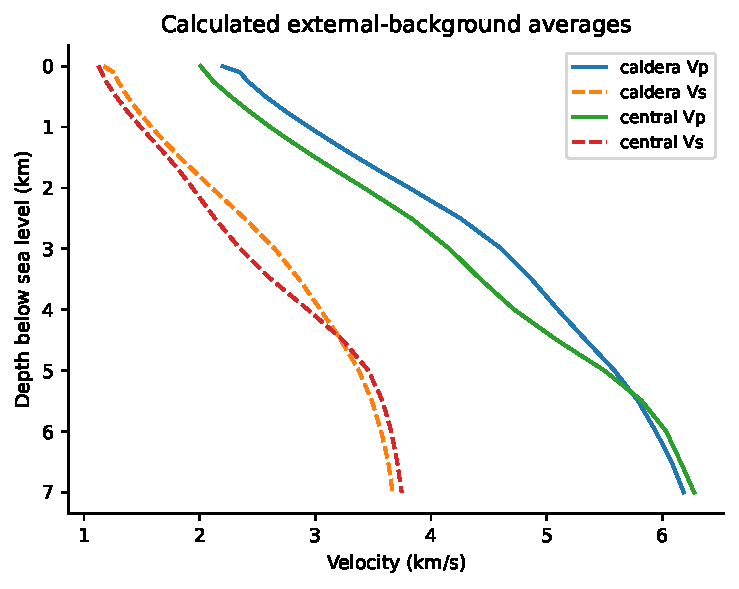
\includegraphics[width=.65\linewidth]{figures/background_profiles.pdf}\caption{Independent averages of the released candidate external background. These calculated profiles are not the authors' fitted 1D model and are not asserted to equal the cited association profile.}\end{figure}
\begin{figure}[p]\centering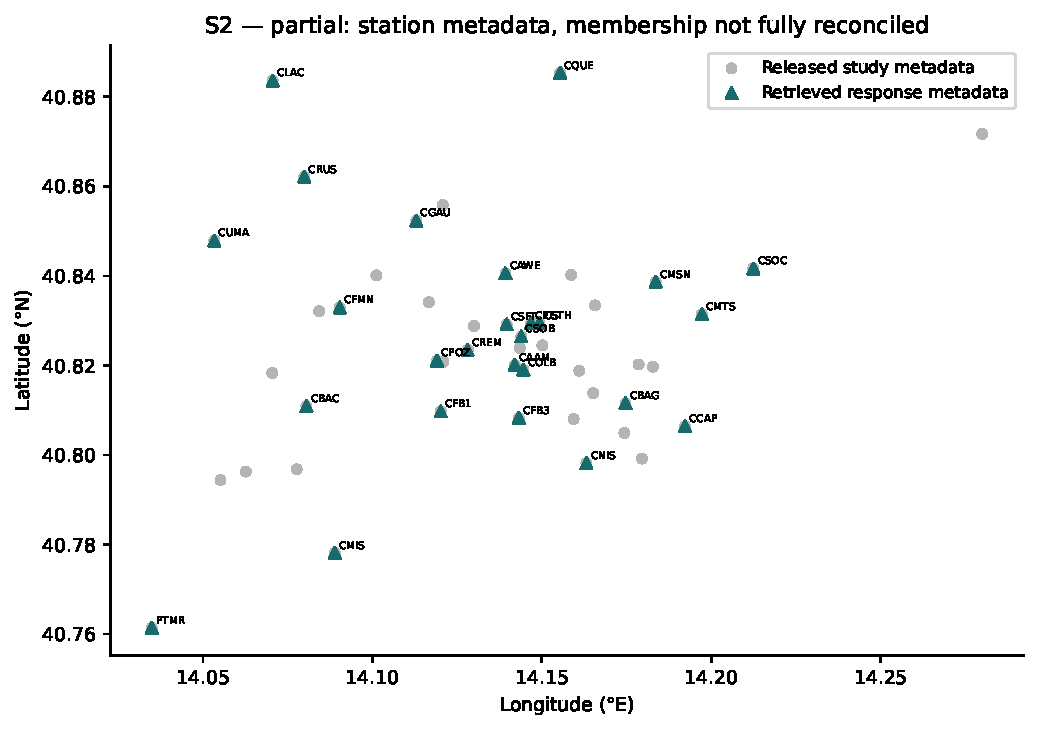
\includegraphics[width=.85\linewidth]{figures/stations_partial.pdf}\caption{S2, partial station inventory. Released station coordinates and independently retrieved IV/2I response metadata. Exact 48-instrument membership, epochs and basemap are not fully reconciled.}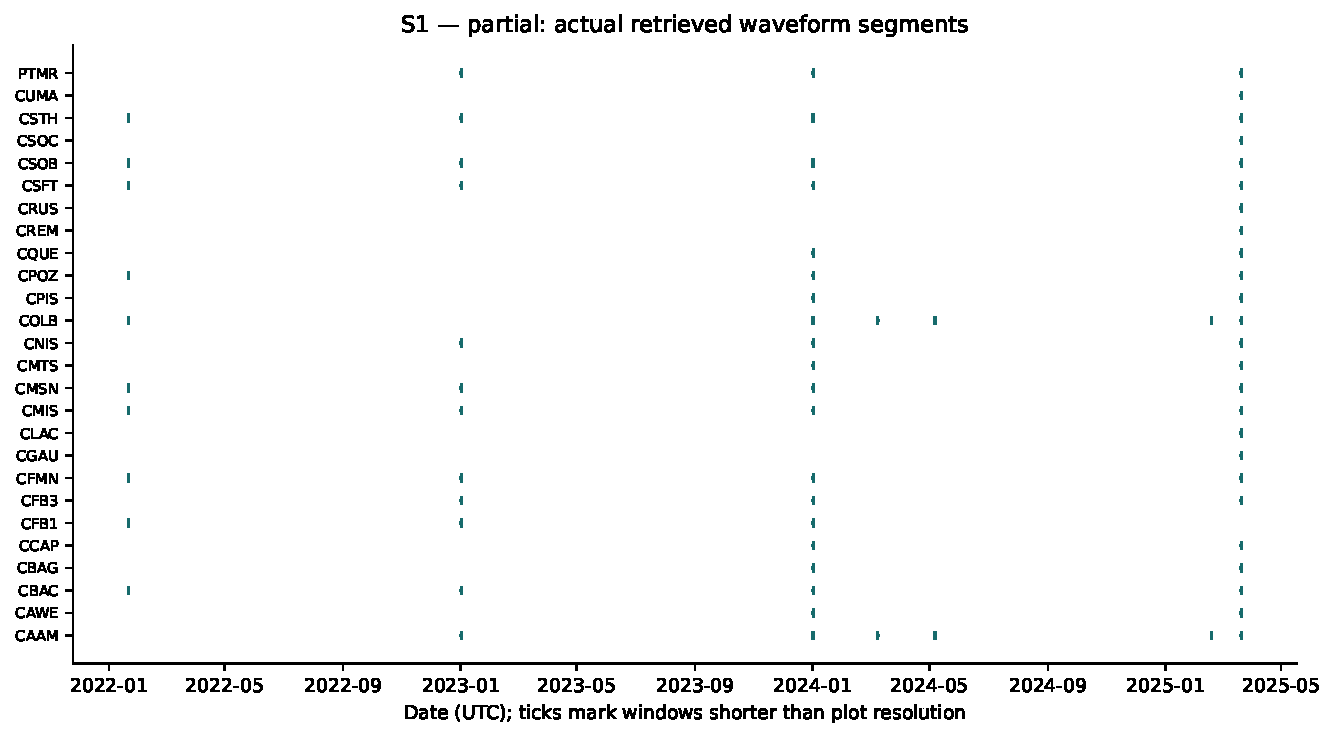
\includegraphics[width=\linewidth]{figures/coverage_partial.pdf}\caption{S1, partial actual returned intervals. Ticks identify retrieved windows shorter than plot resolution. No continuous recording between plotted dates is implied.}\end{figure}
\begin{figure}[p]\centering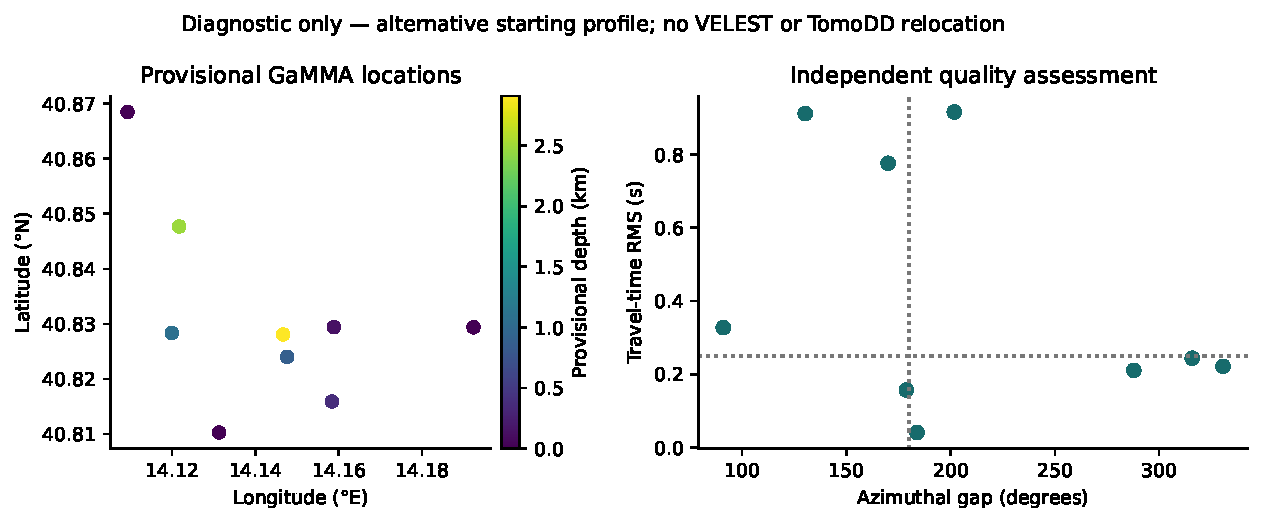
\includegraphics[width=\linewidth]{figures/association_diagnostic.pdf}\caption{New diagnostic, not Figure 3. Provisional associated locations and residual/azimuthal-gap checks. The depth profile differs from the cited initial profile; neither calibrated locations nor TomoDD structures are claimed.}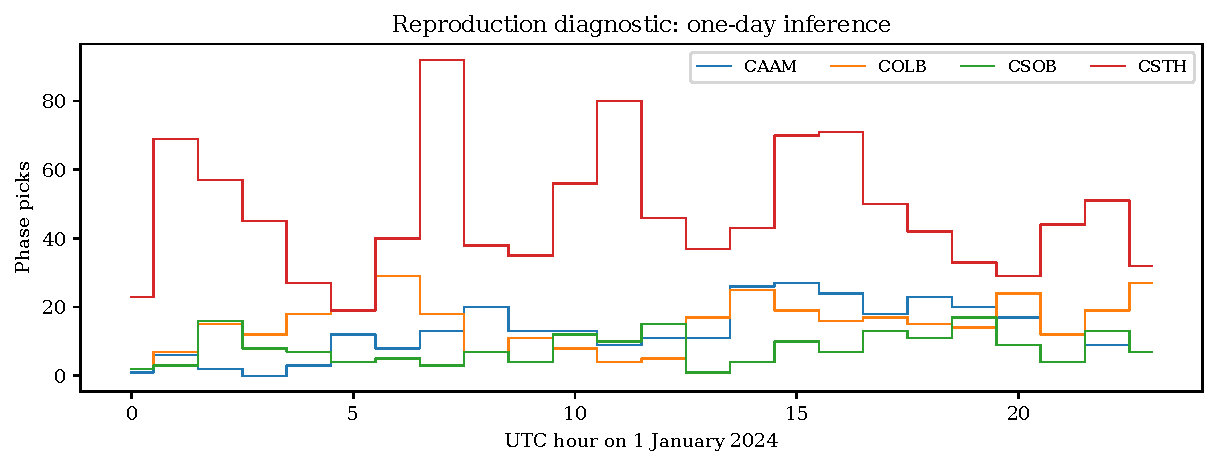
\includegraphics[width=\linewidth]{figures/independent_picks.pdf}\caption{Retained calendar-day pick diagnostic. Model picks are not earthquake counts.}\end{figure}
\begin{figure}[p]\centering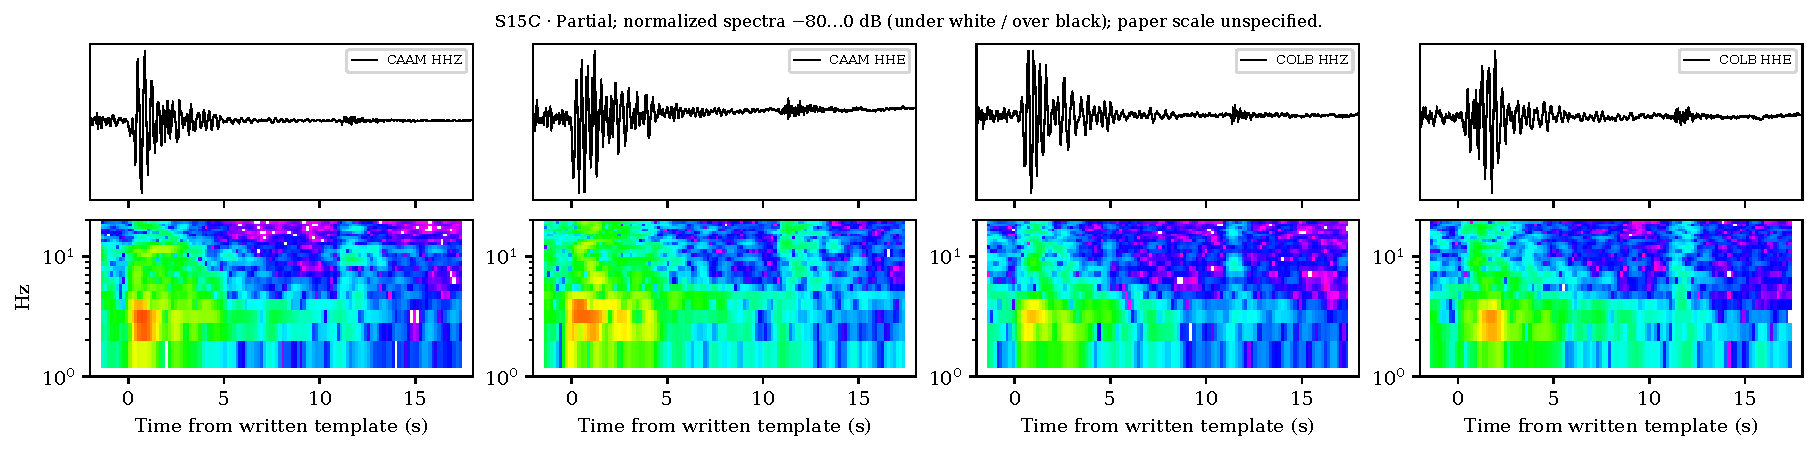
\includegraphics[width=.94\linewidth]{figures/hybrid_E3.pdf}\caption{S15C, partial original-waveform reconstruction. Display normalization, spectral windows and sensitivity correction are explicit assumptions inherited from the retained observational implementation. It is not a source simulation.}\end{figure}
\begin{figure}[p]\centering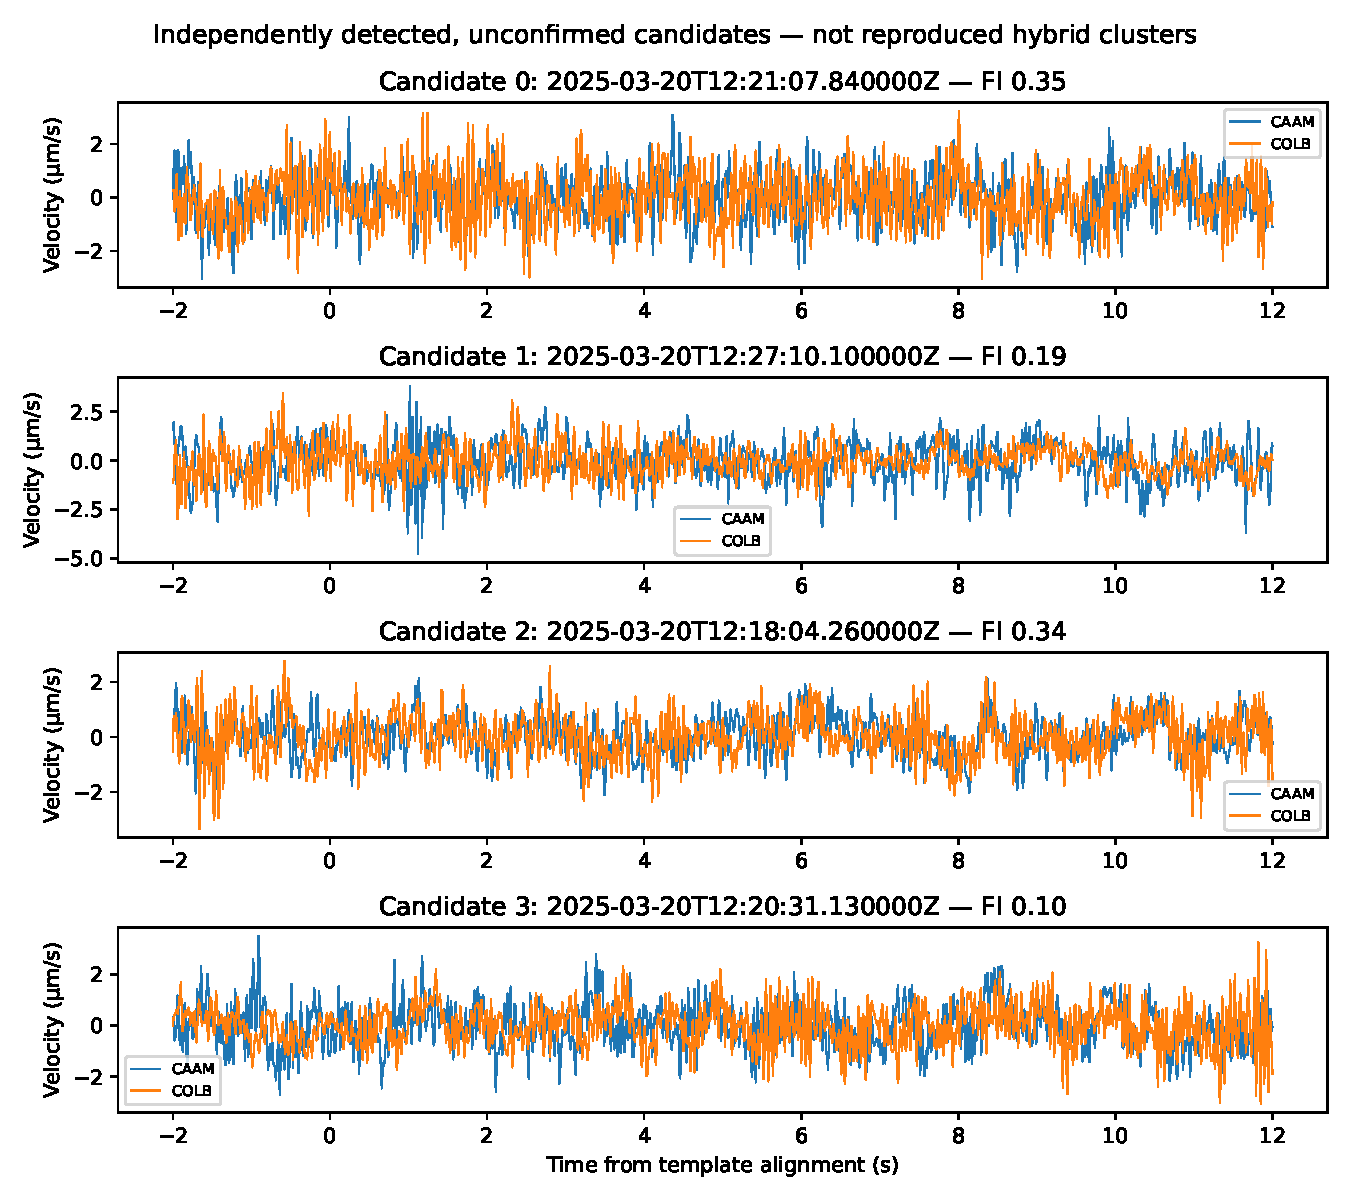
\includegraphics[width=.9\linewidth]{figures/hybrid_candidate_review.pdf}\caption{Independent candidate review. These correlation-threshold crossings remain unconfirmed; their appearance does not establish the paper's hybrid clusters. No supplied hybrid-event list selected these windows.}\end{figure}
\begin{figure}[p]\centering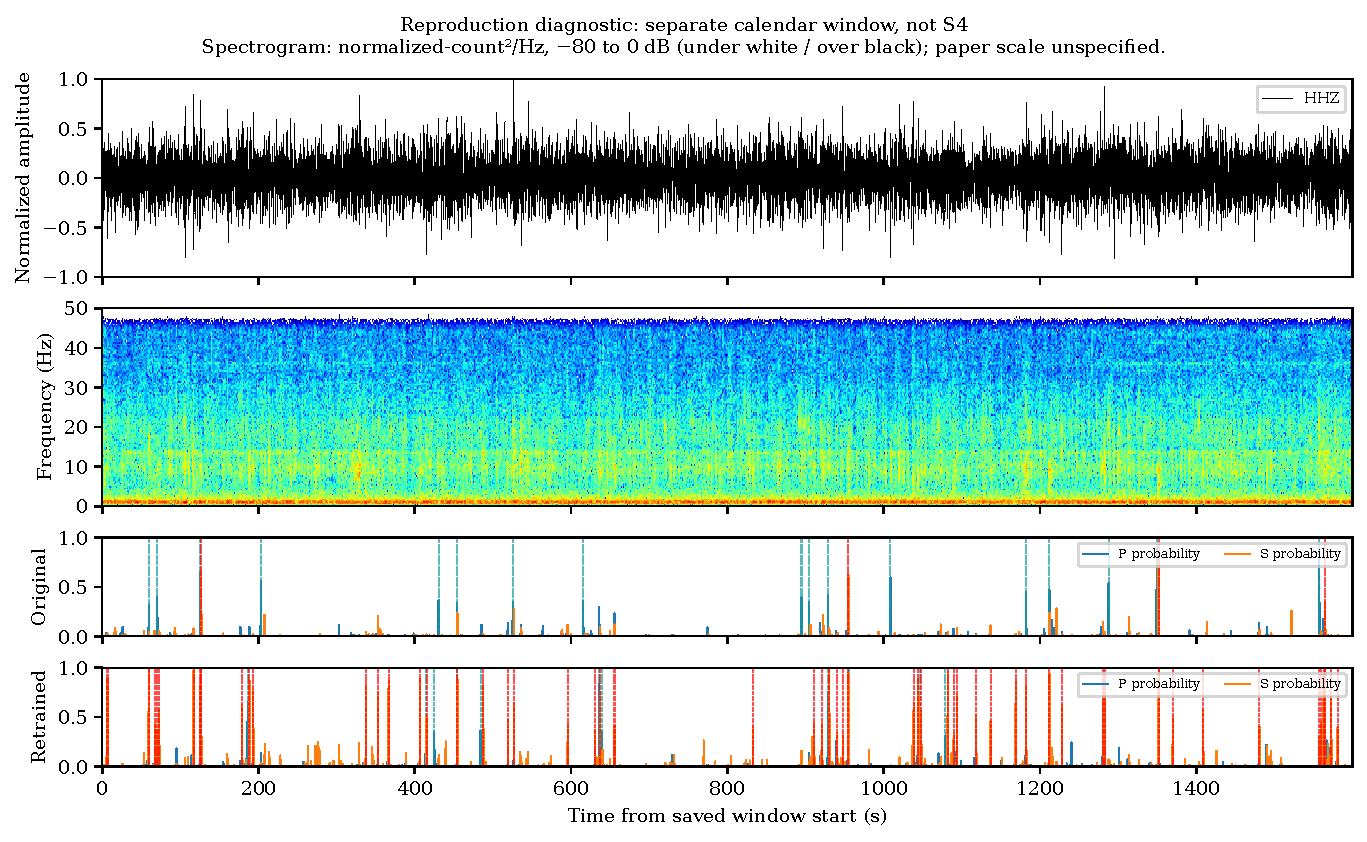
\includegraphics[width=\linewidth]{figures/picker_comparison_CMIS.pdf}\caption{Additional inference comparison on original CMIS observations. The independently calculated probability outputs differ substantially. This is an unlabeled calendar window, not the published S4 example or an accuracy benchmark.}\end{figure}
\begin{figure}[p]\centering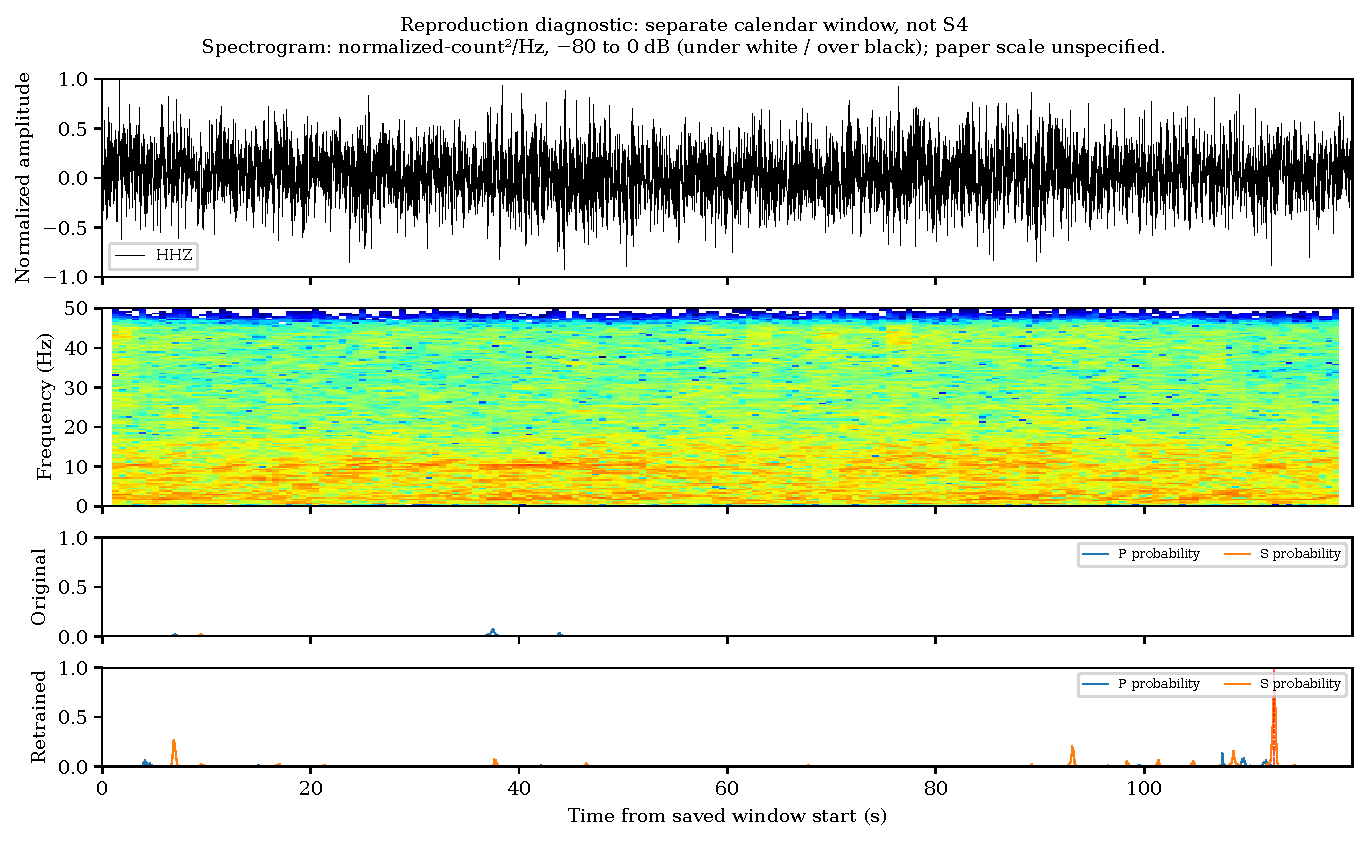
\includegraphics[width=.82\linewidth]{figures/picker_comparison_CSOB.pdf}\caption{Additional original/retrained inference comparison at CSOB on an unlabeled calendar window. Neither the selected time nor the predicted phases is taken from an author catalog.}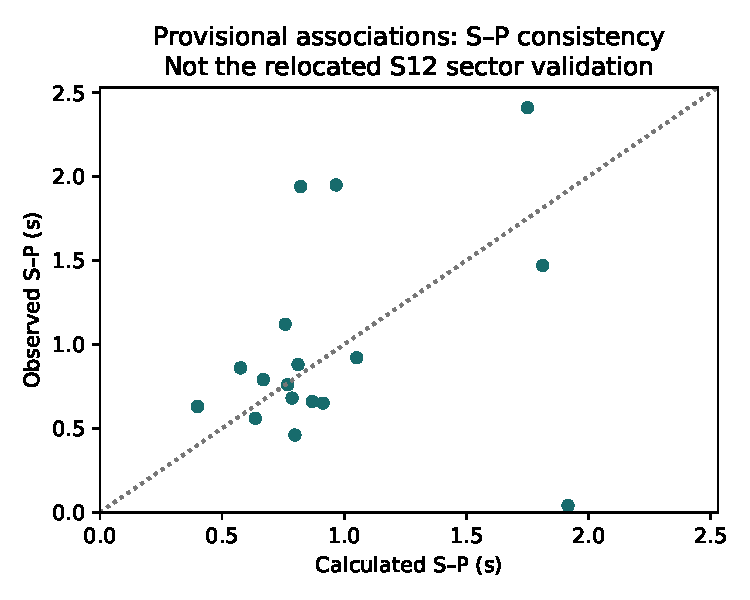
\includegraphics[width=.48\linewidth]{figures/sp_consistency.pdf}\caption{Internal S--P consistency of provisional associations. The dotted line denotes equality. This does not replace S12's relocated sector gathers.}\end{figure}

\clearpage
\section{Completion status and remaining work}
No publication panel is fully independently reproduced. Figure 1B and S1, S2, S15C are partial. All remaining main-text and supplementary panels are not reproduced, including those for which an external context plot is supplied. The full record gives each quantity, written specification, exact inputs, executed data/plot commands or null commands, and a specific limitation. Generic software access is distinguished from scientific execution.

\begin{longtable}{p{.20\linewidth}p{.73\linewidth}}
\toprule Stage & Actual execution and limitation\\\midrule\endhead
1. Collection & Executed calendar windows and whole-period requests; 26 stations retrieved. Full-period chunked download remains unfinished. RAN credentials unavailable.\\[4pt]
2. Phase picking & Executed: 3637 picks; exclusions and merging checked. Full-period inference remains unfinished.\\[4pt]
3. Training / S3--S4 & Retraining not run. STEAD short links return 403; local labels and exact selections/splits missing. Original/retrained inference comparison executed on unlabeled CSOB/CMIS windows, not the exact S4 benchmark.\\[4pt]
4. Association & Executed: 9 provisional events with an alternative external profile. Exact cited numerical starting profile missing; no author event seeds.\\[4pt]
5. VELEST & Generic software compiled. 3 geometry-screened candidates do not resolve the chosen layered model/corrections; inversion not run.\\[4pt]
6. TomoDD & Not run. Independent calibrated input catalog and complete differential-time/configuration workflow missing.\\[4pt]
7. HypoDD SVD & Not run. Depends on independently relocated regional subsets and fitted model; generic software source accessible.\\[4pt]
8. Magnitudes & Measurements executed; 0 qualifying pair equations, 0 calibrated magnitudes. Routine Md permission is resolved.\\[4pt]
9. Completeness / b & Not calculated: no independently calibrated magnitude sample.\\[4pt]
10. Focal mechanisms & Not run. Reviewed polarities, calibrated locations/model and gCAP configuration missing. Generic software accessible. Data S3 row-count discrepancy resolved.\\[4pt]
11. Location checks & Residuals, gaps and internal S--P checks executed. Zero associated CPOZ P arrivals; relocated sector gathers, manual deep-event review and SVD validation unfinished.\\[4pt]
12. Hybrid search & Executed on 24.298 available hours; 4 unconfirmed candidates. Three-year classification, clustering and catalog-wide FI review unfinished.\\[4pt]
13. Historical context & Executed original leveling-table extraction (128 entries) and external routine-catalog context. Original RITE GNSS processed through 2019 with explicit overlap alignment; daily 2020--2023 continuation missing.\\[4pt]
\bottomrule\end{longtable}

The unresolved starting profile, missing acceleration access and incomplete full-period processing are distinct limitations. Lack of a full catalog is not attributed solely to the prompt. Full retrieval, qualified calibration-event selection, VELEST inversion, coherency-weighted differential times, TomoDD relocation, HypoDD uncertainty, reviewed polarities, SKHASH and gCAP inversion, complete magnitude statistics and multiyear hybrid classification remain necessary. Unknown settings require documented assumptions and sensitivity checks rather than hidden substitutions. No coupled physical model is invented.

\section{Rebuild, provenance and replacement}
The README gives environment creation, exact snapshot restoration and the clean rebuild command. The offline rebuild verifies supplied-source and downloaded-input checksums before removing generated products. It reruns the original checks and waveform processing, extended picking/association, analytic association validation, external context extraction, response-corrected amplitude/quality measurements, template scans, plotting, panel tables and two LaTeX passes. Command outcomes are saved in \path{data/build_log.json}. Input hashes and placement URLs are in \path{docs/rebuild_inputs.json}. Live routine pages can change; restoration refuses a mismatched hash and asks for the recorded snapshot or an explicit new provenance audit. Successful HTTP access is not taken as proof of reproducibility of an older mutable archive version.

The previous report source/PDF, station/coverage figures, panel records, input policy, blocker descriptions and rebuild procedure are replaced. Prior observational template figures, raw source documents, independent C++ checks and useful setup are preserved; historical erroneous products remain only in Git history. New outputs are saved under \path{data/extended/}. Exact replacement details are in \path{docs/REPLACEMENTS.md}. This bounded rebuild does not declare the scientific project complete.

All project inputs, environments and intermediate products reside under this repository in \path{inputs/}, \path{.venv/}, \path{tmp/} and \path{build/}. Standard dependency caches may reside in \path{/home/mehffin/.cache/pip}; the earlier initial SeisBench configuration remains in \path{/home/mehffin/.seisbench}. Current analysis redirects SeisBench, plotting and numba caches into the repository. Large inputs and generic software downloads are not committed. Their URLs, sizes, checksums or pinned revisions accompany the project.

\clearpage\appendix
\section{Figure-by-figure record}
The following table records every publication panel or labeled view. For every panel marked not reproduced, no command generates a claimed reproduction; null command fields in the machine-readable record mean unexecuted, not unavailable software. The complete per-panel input paths and command fields are in \href{https://github.com/mehffin-lang/campi-flegrei-independent-reproduction/blob/main/docs/panel_record.json}{\path{docs/panel_record.json}}. Each listed external file's exact URL, size and checksum appears in \path{docs/rebuild_inputs.json}. The partial panels use the recipes below, from the repository root. Each script is invoked with \path{.venv/bin/python scripts/NAME.py}; required upstream outputs are produced by \path{scripts/rebuild.py --clean}.

\begin{itemize}
\item 1B: data \path{context_data.py}; plot \path{plot_extended.py}. Inputs: \path{inputs/extended/delgaudio2010_table.doc}, \path{inputs/extended/demartino_supp.zip} (member \path{RITE_daily.txt}), and \path{inputs/extended/monthly_2023_12.pdf}.
\item S1: data \path{analyze_observations.py} and \path{extended_analysis.py}; plot \path{plot_extended.py}. Inputs: all 171 miniSEED paths explicitly listed in the S1 record and frozen manifest. Actual recorded segments supply the plotted intervals.
\item S2: data \path{analyze_observations.py} and \path{extended_analysis.py}; plot \path{plot_extended.py}. Inputs: \path{inputs/models/stations.csv}, \path{inputs/metadata/channels.txt}, and the 26 XML response files explicitly listed in the S2 record under \path{inputs/extended/responses/}.
\item S15C: data \path{analyze_observations.py}; plot \path{plot_observations.py}. Inputs: \path{inputs/waveforms/E3_CAAM.mseed}, \path{inputs/waveforms/E3_COLB.mseed}, and \path{inputs/metadata/response.xml}.
\end{itemize}
External context recipes for 1A/C and S5 use \path{context_data.py} and \path{plot_extended.py}; the input routine HTML pages are identified row by row in the saved external CSV. Additional diagnostics use \path{compare_pickers.py}, \path{location_consistency.py}, or \path{review_hybrid_candidates.py}, with saved numerical outputs. These commands do not upgrade the corresponding unreproduced publication panels.

\begingroup\footnotesize\begin{longtable}{>{\raggedright\arraybackslash}p{.12\linewidth}>{\raggedright\arraybackslash}p{.25\linewidth}>{\raggedright\arraybackslash}p{.52\linewidth}}
\toprule Panel/view & Quantity & Status, specification and limitation\\\midrule\endhead
1A & INGV event map and large-event markers & partially reproduced. Main p.71, Fig.1 caption. 2005-01-01 to 2025-03-20; origin 14.14 E, 40.82 N; sea-level depth; Md$>$=4 markers Display: depth-colored jet\_r circles, area=0.7+3*10**(Md-2) points squared; missing Md shown as crosses. Exact publication area law unspecified. Full color ranges: 0--8 km for 1A, 0--6 km for S5. Display bounds and off-view counts saved in routine\_plot\_scope.csv.. Current catalog snapshot differs from the historical snapshot: 12,503 located study events versus 12,083. No tuning to published counts. Natural Earth coastline is a display substitute; the original relief/inland-zero contour has not been reconstructed.\\[3pt]
1B & Vertical displacement at Pozzuoli port & partially reproduced. Main p.71, Fig.1 caption. 128 historical entries: 114 leveling surveys, 13 source-provided estimates and one source-provided graphical reconstruction. Source classes preserved separately. Daily GNSS 2000-05-29 through 2025-03-20; median datum from 23 overlapping leveling epochs, +/-15 days. Month-only dates placed on day 15 for display.. Benchmark equivalence and datum-joining convention are assumed because the exact original stitching recipe is not specified. Calendar gaps remain unfilled; no missing recent-data blocker through 2025-03-20.\\[3pt]
1C & Temporal seismicity and cumulative counts & partially reproduced. Main p.71, Fig.1 caption. 2005-2025; cumulative Md$>$0.2; study interval 2022-01-21 to 2025-03-20. Monthly counts and exact-time cumulative Md$>$0.2 reconstructed from the current routine snapshot; historical count differences unresolved. March 2025 is a partial month.\\[3pt]
2A & Catalog seismicity rates by region & not reproduced. Main p.72, Fig.2 caption. Central vs ring/other regions; 54319 vs 12083 catalog events; time bin unspecified. Grid input explicitly authorized; historical transformation and averaging masks not recovered exactly. Local calibration convergence passes, full-path precision and start-model dependence do not. Unreviewed phases and sparse coverage; no accepted relocated scientific catalog. both fixed-grid rounds executed; validation pending\\[3pt]
2B & Depth versus time, symbol size by magnitude & not reproduced. Main p.72, Fig.2 caption. Sea-level depth; near-surface 0-0.5 km; central 0.5-2.1; ring sectors to 3.7 km. Grid input explicitly authorized; historical transformation and averaging masks not recovered exactly. Local calibration convergence passes, full-path precision and start-model dependence do not. Unreviewed phases and sparse coverage; no accepted relocated scientific catalog. both fixed-grid rounds executed; validation pending\\[3pt]
3/\allowbreak{}map & Epicentral spatial pattern & not reproduced. Main p.73, Fig.3 caption. Relative origin 14.14 E, 40.82 N; sea-level depths. Grid input explicitly authorized; historical transformation and averaging masks not recovered exactly. Local calibration convergence passes, full-path precision and start-model dependence do not. Unreviewed phases and sparse coverage; no accepted relocated scientific catalog. both fixed-grid rounds executed; validation pending\\[3pt]
3/\allowbreak{}northing-depth & Depth versus northing & not reproduced. Main p.73, Fig.3 caption. Relative origin 14.14 E, 40.82 N; sea-level depths. Grid input explicitly authorized; historical transformation and averaging masks not recovered exactly. Local calibration convergence passes, full-path precision and start-model dependence do not. Unreviewed phases and sparse coverage; no accepted relocated scientific catalog. both fixed-grid rounds executed; validation pending\\[3pt]
3/\allowbreak{}easting-depth & Depth versus easting & not reproduced. Main p.73, Fig.3 caption. Relative origin 14.14 E, 40.82 N; sea-level depths. Grid input explicitly authorized; historical transformation and averaging masks not recovered exactly. Local calibration convergence passes, full-path precision and start-model dependence do not. Unreviewed phases and sparse coverage; no accepted relocated scientific catalog. both fixed-grid rounds executed; validation pending\\[3pt]
4A & Ring-sector focal mechanisms and seismicity & not reproduced. Main p.74, Fig.4; supplement S6-S7. High quality: SKHASH A or Kagan angle$<$30 deg; gCAP preference with stated exception. Grid input explicitly authorized; historical transformation and averaging masks not recovered exactly. Local calibration convergence passes, full-path precision and start-model dependence do not. Unreviewed phases and sparse coverage; no accepted relocated scientific catalog. both fixed-grid rounds executed; validation pending\\[3pt]
4B & Central/onshore focal mechanisms and seismicity & not reproduced. Main p.74, Fig.4; supplement S6-S7. High quality: SKHASH A or Kagan angle$<$30 deg; gCAP preference with stated exception. Grid input explicitly authorized; historical transformation and averaging masks not recovered exactly. Local calibration convergence passes, full-path precision and start-model dependence do not. Unreviewed phases and sparse coverage; no accepted relocated scientific catalog. both fixed-grid rounds executed; validation pending\\[3pt]
S1 & Station data-availability timeline & partially reproduced. Supplement S12 caption; S2 methods. 48 stations; continuous-data availability. Expanded processed subset: 868 files, 8511.520 channel-hours; full-period queue remains unfinished. No requested-but-failed interval is counted.\\[3pt]
S2 & Station map & partially reproduced. Supplement S13 caption; S2 methods. 23 broadband, 9 short-period, 16 accelerometers. The published 48-instrument membership is not verified. Two released-coordinate pairs coincide; no deployment alias mapping justifies collapsing or removing identifiers.\\[3pt]
S3A & Noise example: waveform, phase labels, spectrogram & not reproduced. Supplement S14 caption; S2-S3. 30-s windows; P/S labels; D amplitude rescaling. Exact training traces and labels not identified from permissible metadata. Retraining was not repeated; permitted trained weights used for inference only.\\[3pt]
S3B & Single-event example: waveform, phase labels, spectrogram & not reproduced. Supplement S14 caption; S2-S3. 30-s windows; P/S labels; D amplitude rescaling. Exact training traces and labels not identified from permissible metadata. Retraining was not repeated; permitted trained weights used for inference only.\\[3pt]
S3C & Two overlapping events: waveform, phase labels, spectrogram & not reproduced. Supplement S14 caption; S2-S3. 30-s windows; P/S labels; D amplitude rescaling. Exact training traces and labels not identified from permissible metadata. Retraining was not repeated; permitted trained weights used for inference only.\\[3pt]
S3D & Five overlapping copies of one event: waveform, phase labels, spectrogram & not reproduced. Supplement S14 caption; S2-S3. 30-s windows; P/S labels; D amplitude rescaling. Exact training traces and labels not identified from permissible metadata. Retraining was not repeated; permitted trained weights used for inference only.\\[3pt]
S4A & Swarms at CSOB: waveform, spectrogram, original and retrained picker scores & partially reproduced. Supplement S15 caption; S2-S3. 120 s CSOB window at 2024-05-20 20:10:03 UTC, interpreting the caption two-hour offset literally; 1 Hz highpass, released model settings, thresholds 0.3.. Exact published start is not specified in the caption; no reference phase labels. Different pick counts do not establish accuracy or successful retraining.\\[3pt]
S4B & CMIS noise: waveform, spectrogram, original and retrained picker scores & not reproduced. Supplement S15 caption; S2-S3. 1600 s; coastal noise; phase threshold 0.3. Original and retrained models both executed on independently selected CSOB/CMIS calendar windows. Exact published windows and independent reference annotations remain unidentified; these diagnostics are not the published benchmark.\\[3pt]
S5/\allowbreak{}map & Routine-catalog spatial views; map & partially reproduced. Supplement S16 caption. 12083 events; 1D model and HYPO71 Display: depth-colored jet\_r circles, area=0.7+3*10**(Md-2) points squared; missing Md shown as crosses. Exact publication area law unspecified. Full color ranges: 0--8 km for 1A, 0--6 km for S5. Display bounds and off-view counts saved in routine\_plot\_scope.csv.. Current catalog snapshot differs from the historical snapshot: 12,503 located study events versus 12,083. No tuning to published counts. Natural Earth coastline is a display substitute; the original relief/inland-zero contour has not been reconstructed.\\[3pt]
S5/\allowbreak{}northing-depth & Routine-catalog spatial views; northing-depth & partially reproduced. Supplement S16 caption. 12083 events; 1D model and HYPO71 Display: depth-colored jet\_r circles, area=0.7+3*10**(Md-2) points squared; missing Md shown as crosses. Exact publication area law unspecified. Full color ranges: 0--8 km for 1A, 0--6 km for S5. Display bounds and off-view counts saved in routine\_plot\_scope.csv.. Current catalog snapshot differs from the historical snapshot: 12,503 located study events versus 12,083. No tuning to published counts. Natural Earth coastline is a display substitute; the original relief/inland-zero contour has not been reconstructed.\\[3pt]
S5/\allowbreak{}easting-depth & Routine-catalog spatial views; easting-depth & partially reproduced. Supplement S16 caption. 12083 events; 1D model and HYPO71 Display: depth-colored jet\_r circles, area=0.7+3*10**(Md-2) points squared; missing Md shown as crosses. Exact publication area law unspecified. Full color ranges: 0--8 km for 1A, 0--6 km for S5. Display bounds and off-view counts saved in routine\_plot\_scope.csv.. Current catalog snapshot differs from the historical snapshot: 12,503 located study events versus 12,083. No tuning to published counts. Natural Earth coastline is a display substitute; the original relief/inland-zero contour has not been reconstructed.\\[3pt]
S6/\allowbreak{}map & Initial-location spatial views; map & not reproduced. Supplement S17 caption. Requires verified fixed 2008 grid, documented regional averages and validated independent VELEST inversions.. Grid input explicitly authorized; historical transformation and averaging masks not recovered exactly. Local calibration convergence passes, full-path precision and start-model dependence do not. Unreviewed phases and sparse coverage; no accepted relocated scientific catalog. both fixed-grid rounds executed; validation pending\\[3pt]
S6/\allowbreak{}northing-depth & Initial-location spatial views; northing-depth & not reproduced. Supplement S17 caption. Requires verified fixed 2008 grid, documented regional averages and validated independent VELEST inversions.. Grid input explicitly authorized; historical transformation and averaging masks not recovered exactly. Local calibration convergence passes, full-path precision and start-model dependence do not. Unreviewed phases and sparse coverage; no accepted relocated scientific catalog. both fixed-grid rounds executed; validation pending\\[3pt]
S6/\allowbreak{}easting-depth & Initial-location spatial views; easting-depth & not reproduced. Supplement S17 caption. Requires verified fixed 2008 grid, documented regional averages and validated independent VELEST inversions.. Grid input explicitly authorized; historical transformation and averaging masks not recovered exactly. Local calibration convergence passes, full-path precision and start-model dependence do not. Unreviewed phases and sparse coverage; no accepted relocated scientific catalog. both fixed-grid rounds executed; validation pending\\[3pt]
S7A/\allowbreak{}map & Cluster locations and 2-sigma errors: map and cross-sectional views; map & not reproduced. Supplement S18 caption; S5 methods. Central174, north165, southwest175, east166; HypoDD SVD; Table S1. Grid input explicitly authorized; historical transformation and averaging masks not recovered exactly. Local calibration convergence passes, full-path precision and start-model dependence do not. Unreviewed phases and sparse coverage; no accepted relocated scientific catalog. both fixed-grid rounds executed; validation pending\\[3pt]
S7A/\allowbreak{}easting-depth & Cluster locations and 2-sigma errors: map and cross-sectional views; easting-depth & not reproduced. Supplement S18 caption; S5 methods. Central174, north165, southwest175, east166; HypoDD SVD; Table S1. Grid input explicitly authorized; historical transformation and averaging masks not recovered exactly. Local calibration convergence passes, full-path precision and start-model dependence do not. Unreviewed phases and sparse coverage; no accepted relocated scientific catalog. both fixed-grid rounds executed; validation pending\\[3pt]
S7B & EX uncertainty versus differential-pick count & not reproduced. Supplement S18 caption. Log-log axes; NCCP+NCCS. Grid input explicitly authorized; historical transformation and averaging masks not recovered exactly. Local calibration convergence passes, full-path precision and start-model dependence do not. Unreviewed phases and sparse coverage; no accepted relocated scientific catalog. both fixed-grid rounds executed; validation pending\\[3pt]
S7D & EY uncertainty versus differential-pick count & not reproduced. Supplement S18 caption. Log-log axes; NCCP+NCCS. Grid input explicitly authorized; historical transformation and averaging masks not recovered exactly. Local calibration convergence passes, full-path precision and start-model dependence do not. Unreviewed phases and sparse coverage; no accepted relocated scientific catalog. both fixed-grid rounds executed; validation pending\\[3pt]
S7F & EZ uncertainty versus differential-pick count & not reproduced. Supplement S18 caption. Log-log axes; NCCP+NCCS. Grid input explicitly authorized; historical transformation and averaging masks not recovered exactly. Local calibration convergence passes, full-path precision and start-model dependence do not. Unreviewed phases and sparse coverage; no accepted relocated scientific catalog. both fixed-grid rounds executed; validation pending\\[3pt]
S7C & EX uncertainty density by cluster & not reproduced. Supplement S18 caption. Kernel density estimate; bandwidth unspecified. Grid input explicitly authorized; historical transformation and averaging masks not recovered exactly. Local calibration convergence passes, full-path precision and start-model dependence do not. Unreviewed phases and sparse coverage; no accepted relocated scientific catalog. both fixed-grid rounds executed; validation pending\\[3pt]
S7E & EY uncertainty density by cluster & not reproduced. Supplement S18 caption. Kernel density estimate; bandwidth unspecified. Grid input explicitly authorized; historical transformation and averaging masks not recovered exactly. Local calibration convergence passes, full-path precision and start-model dependence do not. Unreviewed phases and sparse coverage; no accepted relocated scientific catalog. both fixed-grid rounds executed; validation pending\\[3pt]
S7G & EZ uncertainty density by cluster & not reproduced. Supplement S18 caption. Kernel density estimate; bandwidth unspecified. Grid input explicitly authorized; historical transformation and averaging masks not recovered exactly. Local calibration convergence passes, full-path precision and start-model dependence do not. Unreviewed phases and sparse coverage; no accepted relocated scientific catalog. both fixed-grid rounds executed; validation pending\\[3pt]
S8A & Estimated local versus routine duration magnitude & partially reproduced. Supplement S19 caption; S5-S6 methods. 5 s signal, 2 s preceding noise; SNR $>$=5 dB; all available recorded stations; own picked or predicted P arrivals; $>$=2 shared stations; separation $<$ one fifth of station distance; squared zero-lag correlation weights; Md regularization lambda=1 for unique one-to-one matches within 2 s. Initial locations. B uses 0.1 magnitude bins, maximum-curvature Mc, half-bin-corrected likelihood b and formal Shi-Bolt sampling error; no arbitrary minimum sample cutoff.. 61681 channel measurements, 4705 passing SNR, 1163 relative-amplitude equations, 119 provisional magnitudes. Final relocated locations/full exposure remain missing; routine Md is an allowed regularizer, not independent validation.\\[3pt]
S8B & Magnitude-frequency distribution and fitted b value & partially reproduced. Supplement S19 caption; S6 methods. 5 s signal, 2 s preceding noise; SNR $>$=5 dB; all available recorded stations; own picked or predicted P arrivals; $>$=2 shared stations; separation $<$ one fifth of station distance; squared zero-lag correlation weights; Md regularization lambda=1 for unique one-to-one matches within 2 s. Initial locations. B uses 0.1 magnitude bins, maximum-curvature Mc, half-bin-corrected likelihood b and formal Shi-Bolt sampling error; no arbitrary minimum sample cutoff.. 61681 channel measurements, 4705 passing SNR, 1163 relative-amplitude equations, 119 provisional magnitudes. Final relocated locations/full exposure remain missing; routine Md is an allowed regularizer, not independent validation.\\[3pt]
S9/\allowbreak{}map & Filtered-catalog spatial views and feature labels A-D; map & not reproduced. Supplement S20 caption. 38103 events; NCCP+NCCS threshold 100. Unfinished full-period processing and missing calibrated/relocated catalog. Provisional GaMMA diagnostics use an alternative external profile; they are not this panel. Author-derived results are not substituted.\\[3pt]
S9/\allowbreak{}northing-depth & Filtered-catalog spatial views and feature labels A-D; northing-depth & not reproduced. Supplement S20 caption. 38103 events; NCCP+NCCS threshold 100. Unfinished full-period processing and missing calibrated/relocated catalog. Provisional GaMMA diagnostics use an alternative external profile; they are not this panel. Author-derived results are not substituted.\\[3pt]
S9/\allowbreak{}easting-depth & Filtered-catalog spatial views and feature labels A-D; easting-depth & not reproduced. Supplement S20 caption. 38103 events; NCCP+NCCS threshold 100. Unfinished full-period processing and missing calibrated/relocated catalog. Provisional GaMMA diagnostics use an alternative external profile; they are not this panel. Author-derived results are not substituted.\\[3pt]
S10/\allowbreak{}2022 & Annual seismicity map & not reproduced. Supplement S21 caption. Year 2022. Unfinished full-period processing and missing calibrated/relocated catalog. Provisional GaMMA diagnostics use an alternative external profile; they are not this panel. Author-derived results are not substituted.\\[3pt]
S10/\allowbreak{}2023 & Annual seismicity map & not reproduced. Supplement S21 caption. Year 2023. Unfinished full-period processing and missing calibrated/relocated catalog. Provisional GaMMA diagnostics use an alternative external profile; they are not this panel. Author-derived results are not substituted.\\[3pt]
S10/\allowbreak{}2024 & Annual seismicity map & not reproduced. Supplement S21 caption. Year 2024. Unfinished full-period processing and missing calibrated/relocated catalog. Provisional GaMMA diagnostics use an alternative external profile; they are not this panel. Author-derived results are not substituted.\\[3pt]
S10/\allowbreak{}2025 & Annual seismicity map & not reproduced. Supplement S21 caption. Year 2025 through March20. Unfinished full-period processing and missing calibrated/relocated catalog. Provisional GaMMA diagnostics use an alternative external profile; they are not this panel. Author-derived results are not substituted.\\[3pt]
S11/\allowbreak{}swarm-1 & Map of one of four major swarms & not reproduced. Supplement S22 caption. 2022-2025; exact swarm windows not enumerated in caption. Unfinished full-period processing and missing calibrated/relocated catalog. Provisional GaMMA diagnostics use an alternative external profile; they are not this panel. Author-derived results are not substituted.\\[3pt]
S11/\allowbreak{}swarm-2 & Map of one of four major swarms & not reproduced. Supplement S22 caption. 2022-2025; exact swarm windows not enumerated in caption. Unfinished full-period processing and missing calibrated/relocated catalog. Provisional GaMMA diagnostics use an alternative external profile; they are not this panel. Author-derived results are not substituted.\\[3pt]
S11/\allowbreak{}swarm-3 & Map of one of four major swarms & not reproduced. Supplement S22 caption. 2022-2025; exact swarm windows not enumerated in caption. Unfinished full-period processing and missing calibrated/relocated catalog. Provisional GaMMA diagnostics use an alternative external profile; they are not this panel. Author-derived results are not substituted.\\[3pt]
S11/\allowbreak{}swarm-4 & Map of one of four major swarms & not reproduced. Supplement S22 caption. 2022-2025; exact swarm windows not enumerated in caption. Unfinished full-period processing and missing calibrated/relocated catalog. Provisional GaMMA diagnostics use an alternative external profile; they are not this panel. Author-derived results are not substituted.\\[3pt]
S12A & Ring-sector division & not reproduced. Supplement S23 caption; S8. East, southwest, north; sector boundaries by location/depth. 137 independently associated CPOZ P arrivals now exist. Relocated ring-sector selection and manual depth review remain unfinished; internal S-P checks do not establish location accuracy.\\[3pt]
S12B & Ring-sector division in complementary spatial view & not reproduced. Supplement S23 caption; S8. East, southwest, north; sector boundaries by location/depth. 137 independently associated CPOZ P arrivals now exist. Relocated ring-sector selection and manual depth review remain unfinished; internal S-P checks do not establish location accuracy.\\[3pt]
S12C & Common-receiver gather: east / HHZ & not reproduced. Supplement S23 caption. CPOZ; -1 to +7 s about P; $>$4 Hz; north sector ordered by easting, others northing. 137 independently associated CPOZ P arrivals now exist. Relocated ring-sector selection and manual depth review remain unfinished; internal S-P checks do not establish location accuracy.\\[3pt]
S12D & Common-receiver gather: southwest / HHZ & not reproduced. Supplement S23 caption. CPOZ; -1 to +7 s about P; $>$4 Hz; north sector ordered by easting, others northing. 137 independently associated CPOZ P arrivals now exist. Relocated ring-sector selection and manual depth review remain unfinished; internal S-P checks do not establish location accuracy.\\[3pt]
S12E & Common-receiver gather: north / HHZ & not reproduced. Supplement S23 caption. CPOZ; -1 to +7 s about P; $>$4 Hz; north sector ordered by easting, others northing. 137 independently associated CPOZ P arrivals now exist. Relocated ring-sector selection and manual depth review remain unfinished; internal S-P checks do not establish location accuracy.\\[3pt]
S12F & Common-receiver gather: east / HHN & not reproduced. Supplement S23 caption. CPOZ; -1 to +7 s about P; $>$4 Hz; north sector ordered by easting, others northing. 137 independently associated CPOZ P arrivals now exist. Relocated ring-sector selection and manual depth review remain unfinished; internal S-P checks do not establish location accuracy.\\[3pt]
S12G & Common-receiver gather: southwest / HHN & not reproduced. Supplement S23 caption. CPOZ; -1 to +7 s about P; $>$4 Hz; north sector ordered by easting, others northing. 137 independently associated CPOZ P arrivals now exist. Relocated ring-sector selection and manual depth review remain unfinished; internal S-P checks do not establish location accuracy.\\[3pt]
S12H & Common-receiver gather: north / HHN & not reproduced. Supplement S23 caption. CPOZ; -1 to +7 s about P; $>$4 Hz; north sector ordered by easting, others northing. 137 independently associated CPOZ P arrivals now exist. Relocated ring-sector selection and manual depth review remain unfinished; internal S-P checks do not establish location accuracy.\\[3pt]
S13A & Full caldera seismicity on satellite reference & not reproduced. Supplement S24 caption. Depth-coded relocated events; Google Earth basemap. Unfinished full-period processing and missing calibrated/relocated catalog. Provisional GaMMA diagnostics use an alternative external profile; they are not this panel. Author-derived results are not substituted.\\[3pt]
S13B & Onshore seismicity on satellite reference & not reproduced. Supplement S24 caption. Depth-coded relocated events; Google Earth basemap. Unfinished full-period processing and missing calibrated/relocated catalog. Provisional GaMMA diagnostics use an alternative external profile; they are not this panel. Author-derived results are not substituted.\\[3pt]
S14/\allowbreak{}1 & CAAM waveforms and event annotations & not reproduced. Supplement S25 caption; S9-S11. 1-10 Hz display; 8-s FI at 2-5 and 8-15 Hz; FI$<$0 colored red. 75.797 common CAAM/COLB scan hours; 822 unconfirmed threshold crossings. Three-year scan, reviewed clusters, relative magnitudes and timing histories remain unfinished.\\[3pt]
S14/\allowbreak{}2 & CAAM waveforms and event annotations & not reproduced. Supplement S25 caption; S9-S11. 1-10 Hz display; 8-s FI at 2-5 and 8-15 Hz; FI$<$0 colored red. 75.797 common CAAM/COLB scan hours; 822 unconfirmed threshold crossings. Three-year scan, reviewed clusters, relative magnitudes and timing histories remain unfinished.\\[3pt]
S14/\allowbreak{}3 & CAAM waveforms and event annotations & not reproduced. Supplement S25 caption; S9-S11. 1-10 Hz display; 8-s FI at 2-5 and 8-15 Hz; FI$<$0 colored red. 75.797 common CAAM/COLB scan hours; 822 unconfirmed threshold crossings. Three-year scan, reviewed clusters, relative magnitudes and timing histories remain unfinished.\\[3pt]
S14/\allowbreak{}unclustered & CAAM waveforms and event annotations & not reproduced. Supplement S25 caption; S9-S11. 1-10 Hz display; 8-s FI at 2-5 and 8-15 Hz; FI$<$0 colored red. 75.797 common CAAM/COLB scan hours; 822 unconfirmed threshold crossings. Three-year scan, reviewed clusters, relative magnitudes and timing histories remain unfinished.\\[3pt]
S15A & Hybrid family 1: waveforms and spectrograms & not reproduced. Supplement S26 caption; S9-S10. CAAM/COLB HHZ/HHE; amplitudes normalized by CAAM maximum. Post-generation visual comparison shows a different published example from the written-method template used here. The generated family-template figure is related analysis, not reproduction of this panel.\\[3pt]
S15B & Hybrid family 2: waveforms and spectrograms & not reproduced. Supplement S26 caption; S9-S10. CAAM/COLB HHZ/HHE; amplitudes normalized by CAAM maximum. Post-generation visual comparison shows a different published example from the written-method template used here. The generated family-template figure is related analysis, not reproduction of this panel.\\[3pt]
S15C & Hybrid family 3: waveforms and spectrograms & partially reproduced. Supplement S26 caption; S9-S10. CAAM/COLB HHZ/HHE; amplitudes normalized by CAAM maximum. Written template times used; exact published example alignment, display filtering and spectral settings incompletely specified. Sensitivity-corrected velocities and stated independent display settings used.\\[3pt]
S15D & Shallow volcano-tectonic example: waveforms and spectrograms & not reproduced. Supplement S26 caption; S9-S10. CAAM/COLB HHZ/HHE; amplitudes normalized by CAAM maximum. Exact shallow VT example not identified by written method alone; no author catalog or plot values used to select it.\\[3pt]
\bottomrule\end{longtable}
\endgroup
\section{Equation consistency checks}
\begingroup\small\begin{longtable}{lr r}
\toprule
Check & Absolute error & Tolerance\\\midrule
\endhead
equal\_amplitudes & 0 & 1e-14\\[3pt]
decade\_amplitude & 0 & 1e-14\\[3pt]
ratio\_reversal & 0 & 1e-14\\[3pt]
common\_station\_gain & 5.55e-17 & 1e-14\\[3pt]
zero\_amplitude\_rejected & 0 & 0\\[3pt]
negative\_power\_rejected & 0 & 0\\[3pt]
fi\_mixture\_0 & 4e-15 & 1e-10\\[3pt]
fi\_mixture\_1 & 8.88e-16 & 1e-10\\[3pt]
fi\_mixture\_2 & 1.78e-15 & 1e-10\\[3pt]
fi\_mixture\_3 & 1.55e-15 & 1e-10\\[3pt]
fi\_mixture\_4 & 1.78e-15 & 1e-10\\[3pt]
fi\_mixture\_5 & 2.11e-15 & 1e-10\\[3pt]
fi\_mixture\_6 & 2.22e-16 & 1e-10\\[3pt]
fi\_mixture\_7 & 2.11e-15 & 1e-10\\[3pt]
fi\_mixture\_8 & 1.33e-15 & 1e-10\\[3pt]
fi\_mixture\_9 & 8.88e-16 & 1e-10\\[3pt]
fi\_mixture\_10 & 1.33e-15 & 1e-10\\[3pt]
fi\_mixture\_11 & 4.44e-16 & 1e-10\\[3pt]
fi\_mixture\_12 & 1.78e-15 & 1e-10\\[3pt]
parseval & 3.33e-15 & 1e-10\\[3pt]
fi\_circular\_shift & 7.22e-16 & 1e-10\\[3pt]
fi\_gain & 8.88e-16 & 1e-10\\[3pt]
snr\_5s\_2s\_windows & 8.88e-16 & 1e-10\\[3pt]
magnitude\_exact\_recovery & 1.94e-16 & 1e-12\\[3pt]
magnitude\_pair\_order & 0 & 1e-12\\[3pt]
magnitude\_gauge\_shift & 4.44e-16 & 1e-12\\[3pt]
unanchored\_problem\_rejected & 0 & 0\\[3pt]
\bottomrule
\end{longtable}
\endgroup
\section{Sources}
Primary specification: Tan et al. (2025), Science 390, 70--75, local \path{tanmodel.pdf} and \path{tanmodelsupp.pdf}. Original waveform and response source: \url{https://webservices.ingv.it/fdsnws/}. Required routine magnitude reference and external context: \url{https://terremoti.ov.ingv.it/gossip/flegrei/}. Original leveling table: Del Gaudio et al. (2010), doi:10.1016/j.jvolgeores.2010.05.014, publisher supplement \path{1-s2.0-S0377027310001745-mmc1.doc}. External background references: Battaglia et al. (2008), doi:10.1111/j.1365-2478.2007.00687.x; Cal\`o and Tramelli (2018), doi:10.1038/s41598-018-34456-x. Trained artifact and candidate fixed background release: \url{https://github.com/iamharrison2000/Campi-Flegrei-Earthquake-Monitoring}, revision pinned in the receipts. GaMMA: \url{https://github.com/AI4EPS/GaMMA}, revision \path{80394dd4a4c29450da599f507916ecf1db6203dd}. VELEST: \url{https://seg.ethz.ch/software/velest.html}. Additional source receipts record RAN, temporary observations, STEAD, HypoDD, SKHASH and gCAP. No Tan study-specific analysis or plotting script was used.
\end{document}
